%% Question suisse1
%% simple mc, one correct answer with a figure.
%% figure is small and should be next (right of) to question text.
%% \usepackage{wrapfigure} in preamble.
%% You can 'pull the image up' by adding negative \vspace at the start
%% like in the example. For best effect, put figure definition just in front of question text.
 
\begin{question}{geography-suisse1}

\begin{wrapfigure}{r}{37mm}
  \vspace{-2\baselineskip}
  \begin{center}
    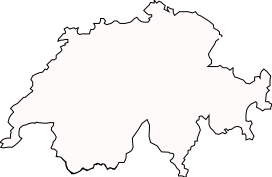
\includegraphics[width=35mm]{\QuestionBaseDir/figures/suisse.pdf}
    \caption{\AMClabel{geography:suisse1}Outline of European country}
  \end{center}
\end{wrapfigure}%
\EN{Which country lies north of Italy, west of Austria, south of Germany
  and east of France and has the shape like in
  figure~\AMCref{geography:suisse1}?}
\NL{Welke land ligt ten noorden van Italië, ten westen van Oostenrijk,
  ten zuiden van Duitsland en ten oosten van Frankrijk en heeft een
  contour zoals in figuur~\AMCref{geography:suisse1}? }
\DE{Weches  Land liegt nördlich Italiens, westlich Österreichs,
  südlich Deutschlands und östlich Frankreichs und hat ein Umriss wie
  in Abbildung~\AMCref{geography:suisse1}? }
  \begin{choices}
    \correctchoice{\EN{Switzerland}\NL{Zwitserland}\DE{Die Schwiez}}
    \wrongchoice{\EN{Austria}\NL{Oostenrijk}\DE{Östereich}}
    \wrongchoice{Monaco}
    \wrongchoice{Liechtenstein}
  \end{choices}
\end{question}


